\scanpage{157}
{\ttfamily\unsure{DATA SETS PICTURE}}
\diagram{\begin{tabular}{|l|l|l|l|l|l|l|l|l|l|l|}
\hline
\ttfamily DDNAME&\ttfamily DESTINATION&\ttfamily CLASS&\ttfamily COPIES&\unsure{\ttfamily RECORDS-NB|RECORD-NB}&\ttfamily BYTES-NB&\ttfamily FORM&\ttfamily FCB&\ttfamily UCS&\ttfamily SPIN&\ttfamily HOLD\\\hline
\ttfamily SYSMSG&\unsure{\ttfamily CNU\quad M6|CNUM06}&A&1&104&\unsure{3936|3856}&\ttfamily STD.&\ttfamily ****&\ttfamily ****& &\\\hline
\end{tabular}}
\[
\begin{aligned}
\rho_s&=\sigma_2\sigma_1\qquad\sigma_1\\
\rho_f&=\sigma_1\sigma_0\qquad\sigma_1=\rho_f\sigma_0\\
\rho_s\rho_f&=\sigma
\end{aligned}
\]
\figure{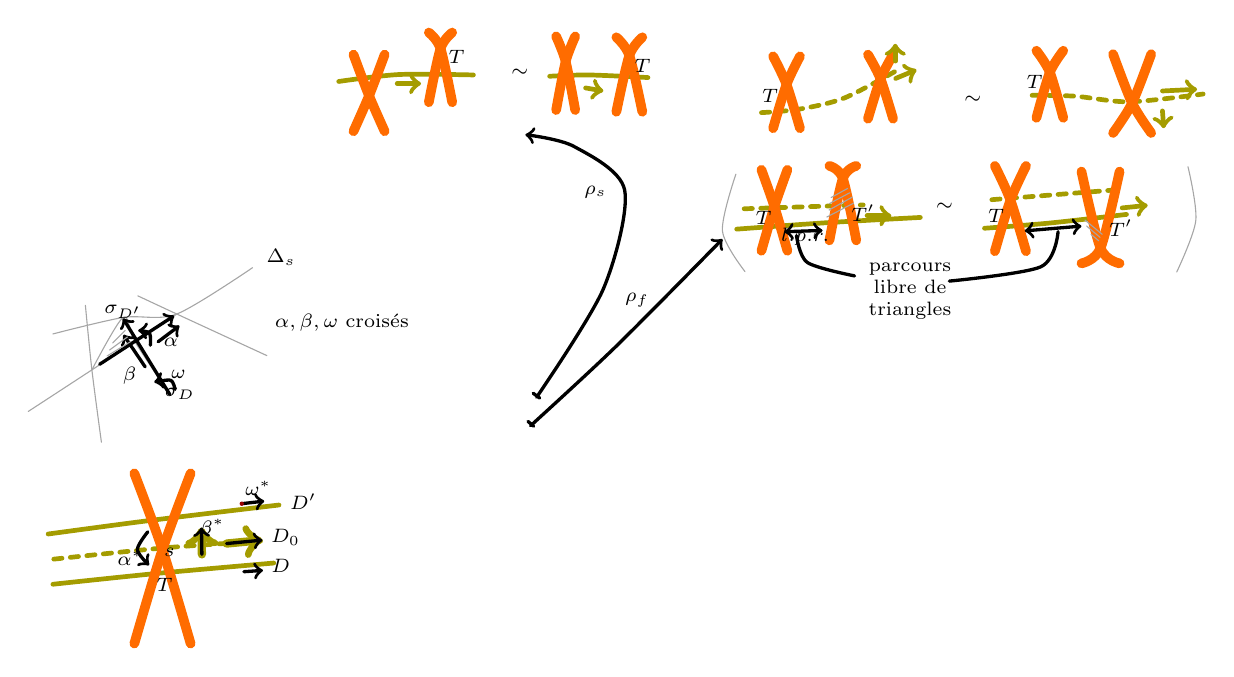
\begin{tikzpicture}[x=.55cm,y=-.55cm,line cap=round,line join=round,g/.style={olive!80!yellow,line width=1.7pt},r/.style={orange!80!brown,line width=1.8pt},w/.style={red!60!black,line width=1.5pt},b/.style={blue!60!black,line width=1.4pt},p/.style={gray!70,thin},k/.style={black,line width=1.2pt},every node/.style={font=\scriptsize}]
\draw[g] plot[smooth] coordinates {(7.97,2.84) (9.36,2.68) (11.08,2.69)};
\draw[orange!85!red,line width=3.5pt] plot[smooth] coordinates {(8.31,2.2199999999999998) (8.67,3.17) (9.03,3.9899999999999998)};
\draw[orange!85!red,line width=3.5pt] plot[smooth] coordinates {(9.03,2.2199999999999998) (8.67,3.17) (8.31,3.9899999999999998)};
\draw[orange!85!red,line width=3.5pt] plot[smooth] coordinates {(10.05,1.71) (10.32,2.08) (10.59,3.3200000000000003)};
\draw[orange!85!red,line width=3.5pt] plot[smooth] coordinates {(10.59,1.71) (10.32,2.08) (10.05,3.3200000000000003)};
\draw[g,->] plot[smooth] coordinates {(9.32,2.89) (9.87,2.89)};
\node at (10.69,2.28) {$T$};
\node at (12.15,2.65) {$\sim$};
\draw[g] plot[smooth] coordinates {(12.84,2.72) (13.74,2.69) (15.11,2.75)};
\draw[orange!85!red,line width=3.5pt] plot[smooth] coordinates {(12.99,1.7999999999999998) (13.21,2.38) (13.430000000000001,3.5)};
\draw[orange!85!red,line width=3.5pt] plot[smooth] coordinates {(13.430000000000001,1.7999999999999998) (13.21,2.38) (12.99,3.5)};
\draw[orange!85!red,line width=3.5pt] plot[smooth] coordinates {(14.379999999999999,1.8200000000000003) (14.68,2.24) (14.98,3.54)};
\draw[orange!85!red,line width=3.5pt] plot[smooth] coordinates {(14.98,1.8200000000000003) (14.68,2.24) (14.379999999999999,3.54)};
\draw[g,->] plot[smooth] coordinates {(13.67,2.99) (14.08,3.06)};
\node at (14.99,2.47) {$T$};
\draw[g,dashed] plot[smooth] coordinates {(17.73,3.56) (18.6,3.48) (19.65,3.22) (20.92,2.55)};
\draw[orange!85!red,line width=3.5pt] plot[smooth] coordinates {(18.0,2.2600000000000002) (18.31,2.91) (18.619999999999997,3.92)};
\draw[orange!85!red,line width=3.5pt] plot[smooth] coordinates {(18.619999999999997,2.2600000000000002) (18.31,2.91) (18.0,3.92)};
\draw[orange!85!red,line width=3.5pt] plot[smooth] coordinates {(20.19,2.2199999999999998) (20.48,2.78) (20.77,3.6999999999999997)};
\draw[orange!85!red,line width=3.5pt] plot[smooth] coordinates {(20.77,2.2199999999999998) (20.48,2.78) (20.19,3.6999999999999997)};
\draw[g,->] plot[smooth] coordinates {(20.82,2.37) (20.82,1.97)};
\draw[g,->] plot[smooth] coordinates {(20.83,2.77) (21.31,2.57)};
\node at (17.93,3.17) {$T$};
\node at (22.61,3.27) {$\sim$};
\draw[g,dashed] plot[smooth] coordinates {(23.98,3.16) (24.97,3.18) (26.23,3.31) (27.93,3.13)};
\draw[orange!85!red,line width=3.5pt] plot[smooth] coordinates {(24.080000000000002,2.13) (24.39,2.63) (24.7,3.6799999999999997)};
\draw[orange!85!red,line width=3.5pt] plot[smooth] coordinates {(24.7,2.13) (24.39,2.63) (24.080000000000002,3.6799999999999997)};
\draw[orange!85!red,line width=3.5pt] plot[smooth] coordinates {(25.849999999999998,2.21) (26.29,3.34) (26.73,4.029999999999999)};
\draw[orange!85!red,line width=3.5pt] plot[smooth] coordinates {(26.73,2.21) (26.29,3.34) (25.849999999999998,4.029999999999999)};
\draw[g,->] plot[smooth] coordinates {(26.99,3.06) (27.79,3.02)};
\draw[g,->] plot[smooth] coordinates {(26.99,3.52) (27.02,3.92)};
\node at (24.04,2.86) {$T$};
\draw[g] plot[smooth] coordinates {(17.16,6.25) (19.26,6.1) (21.4,5.98)};
\draw[g] plot[smooth] coordinates {(22.88,6.23) (24.38,6.11) (26.16,5.91)};
\draw[g,dashed] plot[smooth] coordinates {(17.33,5.78) (20.08,5.69)};
\draw[g,dashed] plot[smooth] coordinates {(23.05,5.57) (25.83,5.35)};
\draw[orange!85!red,line width=3.5pt] plot[smooth] coordinates {(17.73,4.880000000000001) (18.03,5.73) (18.330000000000002,6.75)};
\draw[orange!85!red,line width=3.5pt] plot[smooth] coordinates {(18.330000000000002,4.880000000000001) (18.03,5.73) (17.73,6.75)};
\draw[orange!85!red,line width=3.5pt] plot[smooth] coordinates {(19.3,4.79) (19.61,5.08) (19.919999999999998,6.51)};
\draw[orange!85!red,line width=3.5pt] plot[smooth] coordinates {(19.919999999999998,4.79) (19.61,5.08) (19.3,6.51)};
\draw[orange!85!red,line width=3.5pt] plot[smooth] coordinates {(23.12,4.79) (23.48,5.58) (23.84,6.76)};
\draw[orange!85!red,line width=3.5pt] plot[smooth] coordinates {(23.84,4.79) (23.48,5.58) (23.12,6.76)};
\draw[orange!85!red,line width=3.5pt] plot[smooth] coordinates {(25.119999999999997,4.92) (25.56,6.69) (26.0,7.04)};
\draw[orange!85!red,line width=3.5pt] plot[smooth] coordinates {(26.0,4.92) (25.56,6.69) (25.119999999999997,7.04)};
\draw[p] plot[smooth] coordinates {(19.34,5.52) (19.72,5.31)};
\draw[p] plot[smooth] coordinates {(19.3,5.66) (19.77,5.41)};
\draw[p] plot[smooth] coordinates {(19.29,5.81) (19.83,5.51)};
\draw[p] plot[smooth] coordinates {(19.24,5.97) (19.86,5.65)};
\draw[p] plot[smooth] coordinates {(25.2,6.04) (25.6,6.37)};
\draw[p] plot[smooth] coordinates {(25.24,6.18) (25.55,6.44)};
\draw[p] plot[smooth] coordinates {(25.34,6.37) (25.52,6.52)};
\draw[g,->] plot[smooth] coordinates {(20.17,5.94) (20.73,5.94)};
\draw[g,->] plot[smooth] coordinates {(26.06,5.76) (26.65,5.7)};
\draw[k,<->] plot[smooth] coordinates {(18.26,6.31) (19.14,6.28)};
\draw[k,<->] plot[smooth] coordinates {(23.81,6.29) (25.12,6.18)};
\node at (17.78,6.0) {$T$};
\node at (20.08,5.88) {$T'$};
\node at (23.15,5.94) {$T$};
\node at (26.03,6.23) {$T'$};
\node at (21.96,5.73) {$\sim$};
\node at (18.74,6.43) {$\unsure{l.p.r.}$};
\draw[p] plot[smooth] coordinates {(17.14,4.98) (16.83,6.29) (17.35,7.23)};
\draw[p] plot[smooth] coordinates {(27.58,4.81) (27.76,6.05) (27.32,7.24)};
\draw[k] plot[smooth] coordinates {(18.54,6.4) (18.79,7.02) (19.88,7.33)};
\draw[k] plot[smooth] coordinates {(24.58,6.31) (24.18,7.12) (22.07,7.45)};
\node[align=center] at (21.16,7.69) {parcours\\ libre de\\ triangles};
\draw[k,->] plot[smooth] coordinates {(12.54,10.13) (14.08,7.63) (14.57,5.34) (13.4,4.34) (12.28,4.07)};
\draw[k,->] plot[smooth] coordinates {(12.4,10.79) (14.37,8.96) (16.83,6.48)};
\draw[k] plot[smooth] coordinates {(12.46,10.04) (12.61,10.15)};
\draw[k] plot[smooth] coordinates {(12.34,10.69) (12.47,10.8)};
\node at (13.9,5.39) {$\rho_s$};
\node at (14.86,7.88) {$\rho_f$};
\draw[p] plot[smooth] coordinates {(1.37,8.67) (2.99,8.29) (4.23,8.21) (5.98,7.14)};
\draw[p] plot[smooth] coordinates {(3.33,7.79) (4.23,8.21) (6.31,9.17)};
\draw[p] plot[smooth] coordinates {(2.12,8.01) (2.27,9.5) (2.49,11.17)};
\draw[p] plot[smooth] coordinates {(2.27,9.5) (2.99,8.29) (3.27,8.86) (4.07,10.07)};
\draw[p] plot[smooth] coordinates {(.8,10.46) (2.27,9.5) (4.23,8.21)};
\draw[k,->] plot[smooth] coordinates {(2.45,9.37) (4.17,8.25)};
\draw[k,->] plot[smooth] coordinates {(4.07,10.07) (2.99,8.31)};
\draw[k,->] plot[smooth] coordinates {(3.5,9.43) (3.0,8.69)};
\draw[k,->] plot[smooth] coordinates {(3.8,8.85) (4.29,8.48)};
\draw[k,->] plot[smooth] coordinates {(3.62,8.93) (3.6,8.65) (3.34,8.59)};
\draw[k,->] plot[smooth] coordinates {(4.19,9.95) (4.09,9.74) (3.71,9.78)};
\draw[p] plot[smooth] coordinates {(2.62,9.18) (3.16,8.85)};
\draw[p] plot[smooth] coordinates {(2.68,9.04) (3.09,8.74)};
\draw[p] plot[smooth] coordinates {(2.75,8.88) (3.04,8.59)};
\node at (6.64,6.9) {$\Delta_s$};
\node at (2.99,8.15) {$\sigma_{D'}$};
\node at (4.3,10.06) {$\sigma_D$};
\node at (4.27,9.6) {$\omega$};
\node at (3.14,9.64) {$\beta$};
\node at (4.09,8.86) {$\alpha$};
\node[anchor=west] at (6.27,8.4) {$\alpha,\beta,\omega$ croisés};
\draw[g] plot[smooth] coordinates {(1.26,13.29) (3.59,12.98) (6.59,12.62)};
\draw[g,dashed] plot[smooth] coordinates {(1.39,13.87) (3.94,13.61) (6.24,13.45)};
\draw[g] plot[smooth] coordinates {(1.37,14.45) (3.77,14.2) (6.47,13.96)};
\draw[orange!85!red,line width=3.5pt] plot[smooth] coordinates {(3.25,11.89) (3.9,13.65) (4.55,15.82)};
\draw[orange!85!red,line width=3.5pt] plot[smooth] coordinates {(4.55,11.89) (3.9,13.65) (3.25,15.82)};
\draw[g,->,line width=3pt] plot[smooth] coordinates {(4.81,13.76) (4.8,13.14)};
\draw[g,->,line width=3pt] plot[smooth] coordinates {(5.38,13.51) (6.21,13.43)};
\draw[k,->] plot[smooth] coordinates {(4.81,13.76) (4.8,13.14)};
\draw[k,->] plot[smooth] coordinates {(5.38,13.51) (6.21,13.43)};
\draw[k,->] plot[smooth] coordinates {(5.73,12.59) (6.25,12.53)};
\draw[k,->] plot[smooth] coordinates {(5.78,14.16) (6.22,14.13)};
\draw[k,->] plot[smooth] coordinates {(3.56,13.24) (3.32,13.65) (3.59,14.01)};
\fill[w] (5.73,12.59) circle (.05);
\node at (6.74,13.36) {$D_0$};
\node at (6.63,14.02) {$D$};
\node at (7.15,12.54) {$D'$};
\node at (6.11,12.24) {$\omega^*$};
\node at (5.04,13.17) {$\beta^*$};
\node at (3.16,13.85) {$\alpha^*$};
\node at (4.06,13.72) {$s$};
\node at (3.95,14.46) {$T$};
\end{tikzpicture}}
\diagram{\begin{tikzcd}[ampersand replacement=\&,row sep=2.5em,column sep=3em]
\begin{gathered}\figure{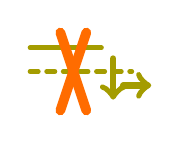
\begin{tikzpicture}[x=.55cm,y=-.55cm,line cap=round,line join=round,g/.style={olive!80!yellow,line width=1.7pt},r/.style={orange!80!brown,line width=1.8pt},w/.style={red!60!black,line width=1.5pt},b/.style={blue!60!black,line width=1.4pt},p/.style={gray!70,thin},k/.style={black,line width=1.2pt},every node/.style={font=\scriptsize}]
\draw[g,dashed] plot[smooth] coordinates {(0,0) (2.35,0)};
\draw[g] plot[smooth] coordinates {(0,-0.55) (1.65,-0.55)};
\draw[orange!85!red,line width=3.5pt] plot[smooth] coordinates {(0.7,-0.9) (1,0) (1.3,0.9)};
\draw[orange!85!red,line width=3.5pt] plot[smooth] coordinates {(1.3,-0.9) (1,0) (0.7,0.9)};
\draw[g,->,line width=2.3pt] plot[smooth] coordinates {(1.92,-0.3) (1.92,0.65)};
\draw[g,->,line width=2.3pt] plot[smooth] coordinates {(2.15,.32) (2.8,.32)};
\end{tikzpicture}}
\\(D_0,-\beta^*,\omega^*)\end{gathered} \& \\
{} \& \begin{gathered}\figure{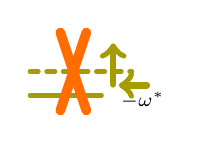
\begin{tikzpicture}[execute at begin node={\ifmmode$\fi},execute at end node={\ifmmode$\fi},x=.55cm,y=-.55cm,line cap=round,line join=round,g/.style={olive!80!yellow,line width=1.7pt},r/.style={orange!80!brown,line width=1.8pt},w/.style={red!60!black,line width=1.5pt},b/.style={blue!60!black,line width=1.4pt},p/.style={gray!70,thin},k/.style={black,line width=1.2pt},every node/.style={font=\scriptsize}]
\draw[g,dashed] plot[smooth] coordinates {(0,0) (2.35,0)};
\draw[g] plot[smooth] coordinates {(0,0.55) (1.65,0.55)};
\draw[orange!85!red,line width=3.5pt] plot[smooth] coordinates {(0.7,-0.9) (1,0) (1.3,0.9)};
\draw[orange!85!red,line width=3.5pt] plot[smooth] coordinates {(1.3,-0.9) (1,0) (0.7,0.9)};
\draw[g,->,line width=2.3pt] plot[smooth] coordinates {(1.92,0.3) (1.92,-0.65)};
\draw[g,->,line width=2.3pt] plot[smooth] coordinates {(2.7,.32) (2.05,.32)};
\node at (2.6,.67) {$-\omega^*$};
\end{tikzpicture}}
\\(D_0,\beta^*,-\omega^*)\end{gathered} \\
(D_0,\beta^*\omega^*) \arrow[uu,"\sigma",mapsto] \arrow[ur,"\sigma_0",mapsto] \arrow[r,"\sigma_1",mapsto] \arrow[dr,"\sigma_2",mapsto] \& \figure{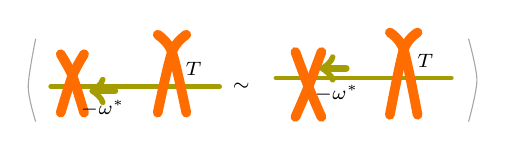
\begin{tikzpicture}[execute at begin node={\ifmmode$\fi},execute at end node={\ifmmode$\fi},x=.55cm,y=-.55cm,line cap=round,line join=round,g/.style={olive!80!yellow,line width=1.7pt},r/.style={orange!80!brown,line width=1.8pt},w/.style={red!60!black,line width=1.5pt},b/.style={blue!60!black,line width=1.4pt},p/.style={gray!70,thin},k/.style={black,line width=1.2pt},every node/.style={font=\scriptsize}]
\draw[g] plot[smooth] coordinates {(0,0) (3.9,0)};
\draw[orange!85!red,line width=3.5pt] plot[smooth] coordinates {(0.22999999999999998,-0.75) (0.5,-0.25) (0.77,0.6)};
\draw[orange!85!red,line width=3.5pt] plot[smooth] coordinates {(0.77,-0.75) (0.5,-0.25) (0.22999999999999998,0.6)};
\draw[orange!85!red,line width=3.5pt] plot[smooth] coordinates {(2.4699999999999998,-1.2000000000000002) (2.8,-0.8) (3.13,0.5999999999999999)};
\draw[orange!85!red,line width=3.5pt] plot[smooth] coordinates {(3.13,-1.2000000000000002) (2.8,-0.8) (2.4699999999999998,0.5999999999999999)};
\draw[g,<-,line width=2.5pt] plot[smooth] coordinates {(.89,.1) (1.48,.1)};
\node at (1.2,.5) {$-\omega^*$};
\node at (3.3,-.4) {$T$};
\node at (4.4,0) {$\sim$};
\draw[g] plot[smooth] coordinates {(5.2,-.2) (9.25,-.2)};
\draw[orange!85!red,line width=3.5pt] plot[smooth] coordinates {(5.65,-0.8) (5.95,0) (6.25,0.7)};
\draw[orange!85!red,line width=3.5pt] plot[smooth] coordinates {(6.25,-0.8) (5.95,0) (5.65,0.7)};
\draw[orange!85!red,line width=3.5pt] plot[smooth] coordinates {(7.83,-1.25) (8.15,-0.85) (8.47,0.65)};
\draw[orange!85!red,line width=3.5pt] plot[smooth] coordinates {(8.47,-1.25) (8.15,-0.85) (7.83,0.65)};
\draw[g,<-,line width=2.5pt] plot[smooth] coordinates {(6.2,-.42) (6.82,-.42)};
\node at (6.6,.15) {$-\omega^*$};
\node at (8.65,-.6) {$T$};
\draw[p] plot[smooth] coordinates {(-.35,-1.1) (-.52,0) (-.35,.8)};
\draw[p] plot[smooth] coordinates {(9.65,-1.1) (9.84,-.15) (9.65,.8)};
\end{tikzpicture}}
 \\
\& \begin{gathered}\figure{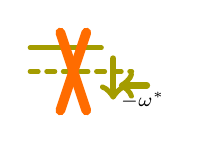
\begin{tikzpicture}[execute at begin node={\ifmmode$\fi},execute at end node={\ifmmode$\fi},x=.55cm,y=-.55cm,line cap=round,line join=round,g/.style={olive!80!yellow,line width=1.7pt},r/.style={orange!80!brown,line width=1.8pt},w/.style={red!60!black,line width=1.5pt},b/.style={blue!60!black,line width=1.4pt},p/.style={gray!70,thin},k/.style={black,line width=1.2pt},every node/.style={font=\scriptsize}]
\draw[g,dashed] plot[smooth] coordinates {(0,0) (2.35,0)};
\draw[g] plot[smooth] coordinates {(0,-0.55) (1.65,-0.55)};
\draw[orange!85!red,line width=3.5pt] plot[smooth] coordinates {(0.7,-0.9) (1,0) (1.3,0.9)};
\draw[orange!85!red,line width=3.5pt] plot[smooth] coordinates {(1.3,-0.9) (1,0) (0.7,0.9)};
\draw[g,->,line width=2.3pt] plot[smooth] coordinates {(1.92,-0.3) (1.92,0.65)};
\draw[g,->,line width=2.3pt] plot[smooth] coordinates {(2.7,.32) (2.05,.32)};
\node at (2.6,.67) {$-\omega^*$};
\end{tikzpicture}}
\\(D_0,-\beta^*,-\omega^*)\end{gathered}
\end{tikzcd}}

$\alpha^*,\beta^*,\omega^*$ \uline{non} croisés
\[
\omega^*=-\alpha^*\wedge\beta^*\qquad
\omega=\alpha\wedge\beta
\]
$\sigma_0$ donc change $\alpha$ en $-\alpha$, en gardant $\sigma_D,\sigma_{D'},\beta$.

$\sigma_2$ échange $\sigma_D$ et $\sigma_{D'}$, change $\beta$ en $-\beta$, garde $\alpha$.
\margin{\mspage{156}}
